% ---
% filename : ["electrotechnique_circuits_dc_20260429_986_resistance_interne_pile.tex"]
% id : "electrotechnique_circuits_dc_20260429_986"
% title : "Résistance interne d'une pile"
% domain : "Électrotechnique"
% subdomain : "Circuits DC"
% tags : ["pile", "résistance interne", "loi d'Ohm", "circuit série", "ts"]
% difficulty : 1
% time_solve : 2
% has_octave : True
% octave_files : ["electrotechnique_circuits_dc_20260429_986_resistance_interne_pile.m"]
% author : "om"
% ---
\documentclass[a4paper,11pt,answers,addpoints]{exam}

% ---------------------------------------------------------
% LANGUE, ENCODAGE, FONTS
% ---------------------------------------------------------
\usepackage[utf8]{inputenc}

% ---------------------------------------------------------
% GÉOMÉTRIE ET MISE EN PAGE
% ---------------------------------------------------------
\usepackage[left=1.7cm,right=1.5cm,top=2cm,bottom=1cm]{geometry}
%\usepackage{a4wide}

% ---------------------------------------------------------
% MATHÉMATIQUES
% ---------------------------------------------------------
\usepackage{amsmath, amssymb, bm, esvect}

% Vecteurs
\newcommand{\V}{\overrightarrow}
\def\vect#1{\overrightarrow{\strut#1}}
\providecommand{\Degrees}[0]{\ensuremath{^\circ}}

% ---------------------------------------------------------
% UNITÉS ET GRANDEURS (SIunitx)
% ---------------------------------------------------------
\usepackage{siunitx}
\sisetup{output-decimal-marker={,}}
\DeclareSIUnit \var {var}
\DeclareSIUnit \VA {VA}
\DeclareSIUnit \kVA {kVA}
\DeclareSIUnit[quantity-product={}] \degree{\text{\textdegree}}

% ---------------------------------------------------------
% GRAPHIQUES : TikZ + CircuitikZ + PGFPlots
% ---------------------------------------------------------
\usepackage{tikz}
\usetikzlibrary{
	arrows.meta,
	intersections,
	decorations.pathreplacing,
	positioning
}

\usepackage[european,straightvoltages,EFvoltages]{circuitikz}

\usepackage{tkz-fct}
\usepackage{pgfplots}
\pgfplotsset{compat=1.12}

% Symbole étoile-triangle personnalisé
\newcommand{\wye}{%
	\mathbin{\tikz[x=1ex,y=1ex]{%
			\draw[line width=.1ex] (0,0)--(45:1)--++(-45:1) (45:1)--++(0,1);
	}}%
}

% ---------------------------------------------------------
% TABLEAUX
% ---------------------------------------------------------
\usepackage{tabularx}
\usepackage{tabu}

% ---------------------------------------------------------
% HYPERLIENS
% ---------------------------------------------------------
\usepackage[colorlinks=true,
menucolor=red,
breaklinks=true,
urlcolor=blue,
linkcolor=blue]{hyperref}

% ---------------------------------------------------------
% COMMANDES PERSONNELLES
% ---------------------------------------------------------
\newcommand\nomauteur{bdminasmorgul@protonmail.com}
\newcommand\dateTe{29.04.2026}
\newcommand\brancheTe{TS}

% ---------------------------------------------------------
% STYLE DE L'EXERCICE
% ---------------------------------------------------------
\pagestyle{headandfoot}
\firstpageheadrule
\runningheadrule

\firstpageheader{\brancheTe\ (\nomauteur)}{Élève : }{(\dateTe) \thepage/\numpages}
\runningheader{\brancheTe\ (\nomauteur)}{Élève : }{(\dateTe) \thepage/\numpages}

% Compteur en bas de page
\newcommand{\totalpointtts}{%
	\begin{tikzpicture}[remember picture, overlay]
		\node[anchor=south west, inner sep=0pt, outer sep=0pt]
		at ([xshift=0.5cm,yshift=0.5cm]current page.south west)
		{\rotatebox{90}{Total des points : \numpoints}};
	\end{tikzpicture}
}

\firstpagefooter{\totalpointtts}{}{}
\runningfooter{\totalpointtts}{}{}

% Réglages exam
\printanswers
\addpoints
\pointsinmargin
\bracketedpoints

% ---------------------------------------------------------
% LISTINGS (code)
% ---------------------------------------------------------
\usepackage{xcolor}
\usepackage{listings}

\lstdefinestyle{octavestyle}{
	language=Matlab,
	basicstyle=\ttfamily\small,
	keywordstyle=\color{blue},
	commentstyle=\color{green!50!black},
	stringstyle=\color{red},
	stepnumber=1,
	frame=single,
	breaklines=true,
	breakatwhitespace=true,
	tabsize=4
}

% ---------------------------------------------------------
% DOCUMENT
% ---------------------------------------------------------
\begin{document}
	
	
	\unframedsolutions
	\pointsinmargin
	\bracketedpoints
	\section*{Préparation TS PQ CFC ELMO, IELE, PELE}
	\begin{questions}

\question[6]
Soit une pile avec une tension $U_0$ et une charge résistive $R_{ch}$, le courant qui traverse la charge est donné. Calculer la valeur de sa résistance interne $R_{int} \qty{}{[\ohm]}$\\
Données numériques~: \ $U_0 = \qty{1.5}{[\volt]}; R_{ch} = \qty{2}{[\ohm]}$; I = \qty{0.15}{[\ampere]}\\
\vspace*{0.5cm}
\begin{center}
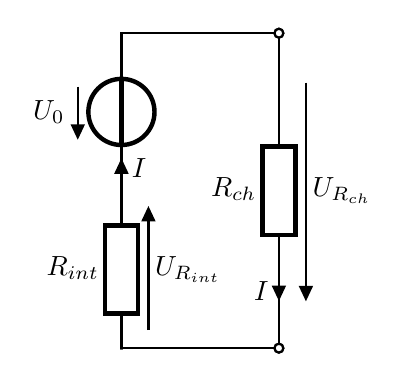
\begin{tikzpicture}[thick,x=1cm, y=1cm]
	% Grille de fond
	%	\tikzset{OMdeYLB/.style={help lines,color=green!50}}
	%	\draw[OMdeYLB] (-2,-1) grid (10,8);
	
	% Étiquettes sur les axes X et Y
	%	\foreach \x in {-2,-1,...,10}
	%	\node[below, font=\tiny, red!70] at (\x,-1) {\x};
	
	%	\foreach \y in {-1,0,...,4}
	%	\pgfmathtruncatemacro{\yc}{int(2*\y)}
	%	\node[left, font=\tiny, red!70] at (-2,\yc) {\yc};	
	% --- Grille auto ---
	\foreach \x in {0,0.5,...,8}{
		\foreach \y in {0,0.5,...,7}{
			\pgfmathtruncatemacro{\xx}{int(2*\x)}
			\pgfmathtruncatemacro{\yy}{int(2*\y)}
			\coordinate (N\xx\yy) at (\x,\y);
		}
	}
	
	
	% --- Lignes des phases existantes ---
	%	\draw (N012) node[left] {L1} -- (N412);
	%	\draw (N010) node[left] {L2} -- (N410);
	%	\draw (N08) node[left] {L3} -- (N48);
	
	% ==========================================================
	%           REPRODUCTION DU CIRCUIT AVEC LA GRILLE
	% ==========================================================
	
	%	\begin[circuitikz, european, thick]
	%		\ctikzset {bipole/name}.-300
	%		\ctikzset {voltage/distance from line=0.2}
	%		\ctikzset {voltage/bump a=.9}
	%		\ctikzset {voltage/bump b=2.2}
	%		\ctikzset{voltage/european label distance = 2.2}
	%		\ctikzset{current/distance = 1.8}
	
	% --- Source verticale ---
	\draw (N04) to[V,i>_=$I$, v<=$U_0$,.-.] (N08);
	
	% --- Résistance horizontale ---
	\draw (N00) to[R, l^=$R_{int}$, v_>=$U_{R_{int}}$,.-.] (N04);
	%		node[above] {JE};
	
	% --- Fil bas avec borne AN ---
	\draw (N08) to[short,.-o] (N48);
	\draw (N00) to[short,.-o] (N40);	
	%		node[below] {AN};
	
	\draw (N48) to[R,l_=$R_{ch}$, v^=$U_{R_{ch}}$, i_=$I$, o-o] (N40);
	% --- Court-circuit vertical droite ---
	%		\draw (N808) to[short,o-o] (N800);
	
	% --- Tensions mesurées U_LOL et U_JEAN ---
	%		\draw ([xshift=-4pt]N000) 
	%		to [open, v^<=$U_{LOL}$] 
	%		([xshift=-4pt]N008);
	
	%		\draw ([xshift=0pt]N808)
	%		to [open, v^>=$U_{JEAN}$]
	%		([xshift=0pt]N800);
	
	
	
\end{tikzpicture}
\end{center}

\begin{solution} 
	\begin{align*} 
		R_{tot} &= \dfrac{U_0}{I} = \dfrac{1.5}{0.15} = \qty{10}{[\ohm]}\\[6pt] 
		R_{int} &= R_{tot} - R_{ch} = \num{10} - \num{2} = \qty{8}{[\ohm]}\\[6pt]
		\text{Autre solution~:}\\
		U_{R_{ch}} &= R_{ch} \cdot I = \num{2} \cdot \num{0.15} = \qty{0.3}{[\volt]}\\[6pt] 
		U_{R_{int}} &= U_0 - U_{R_{ch}} = \num{1.5} - \num{0.3} = \qty{1.2}{[\volt]}\\
		R_{int} &= \dfrac{U_{R_{int}}}{I} = \dfrac{1.2}{0.15} = \qty{8}{[\ohm]}
	\end{align*}
	\begin{verbatim} 
		% Télécharger OCTAVE depuis https://wiki.octave.org/Using_Octave et l'installer 
		% Puis copier-coller le code dans OCTAVE
		
		% Données du projet 
		Em = 750;  % Éclairement requis [lux] 
		longueur = 15;      % [m] 
		largeur = 8;        % [m] 
		eta = 0.6;          % Rendement global (facteur maintenance inclus) 
		phi_L = 8500;       % Flux d'un luminaire [lm]
		
		% Calcul de la surface A = longueur * largeur;
		% Calcul du nombre théorique de luminaires 
		n_theo = (Em * A) / (phi_L * eta);
		% Arrondi à l'entier supérieur 
		n_reel = ceil(n_theo);
		% Affichage des résultats 
		printf("Surface à éclairer : %.2f [m^2]\n", A); 
		printf("Nombre théorique de luminaires : %.2f\n", n_theo); 
		printf("Nombre de luminaires à installer : %d\n", n_reel); 
		printf("Éclairement final estimé : %.2f [lux]\n", (n_reel * phi_L * eta) / A); 
	\end{verbatim} 
\end{solution}
\end{questions}
\end{document}
